\chapter{Análisis de los resultados}
\label{resultados}

A lo largo de este capitulo se va a tratar de analizar, comparar y discutir los resultados obtenidos mediante HFSS sobre los diseños que se comentaron en la sección \ref{analdis}. Se analizará cada configuración por separado y se mostrarán las gráficas y valores principales para cada una de las configuraciones de 2GHz y 6 GHz y finalmente la configuración a 27 GHz. No se analizará el caso del parche simple a 2.4 GHz puesto que ya fue analizado detalladamente en la sección \ref{procesodiseno}.

\section{Parche Simple a 6 GHz}
\subsection{Pérdidas de retorno}
\par Comenzaremos analizando la curva de pérdidas de retorno o parámetro S del parche simple a 6 GHz. 

\begin{figure}[h]
    \centering
        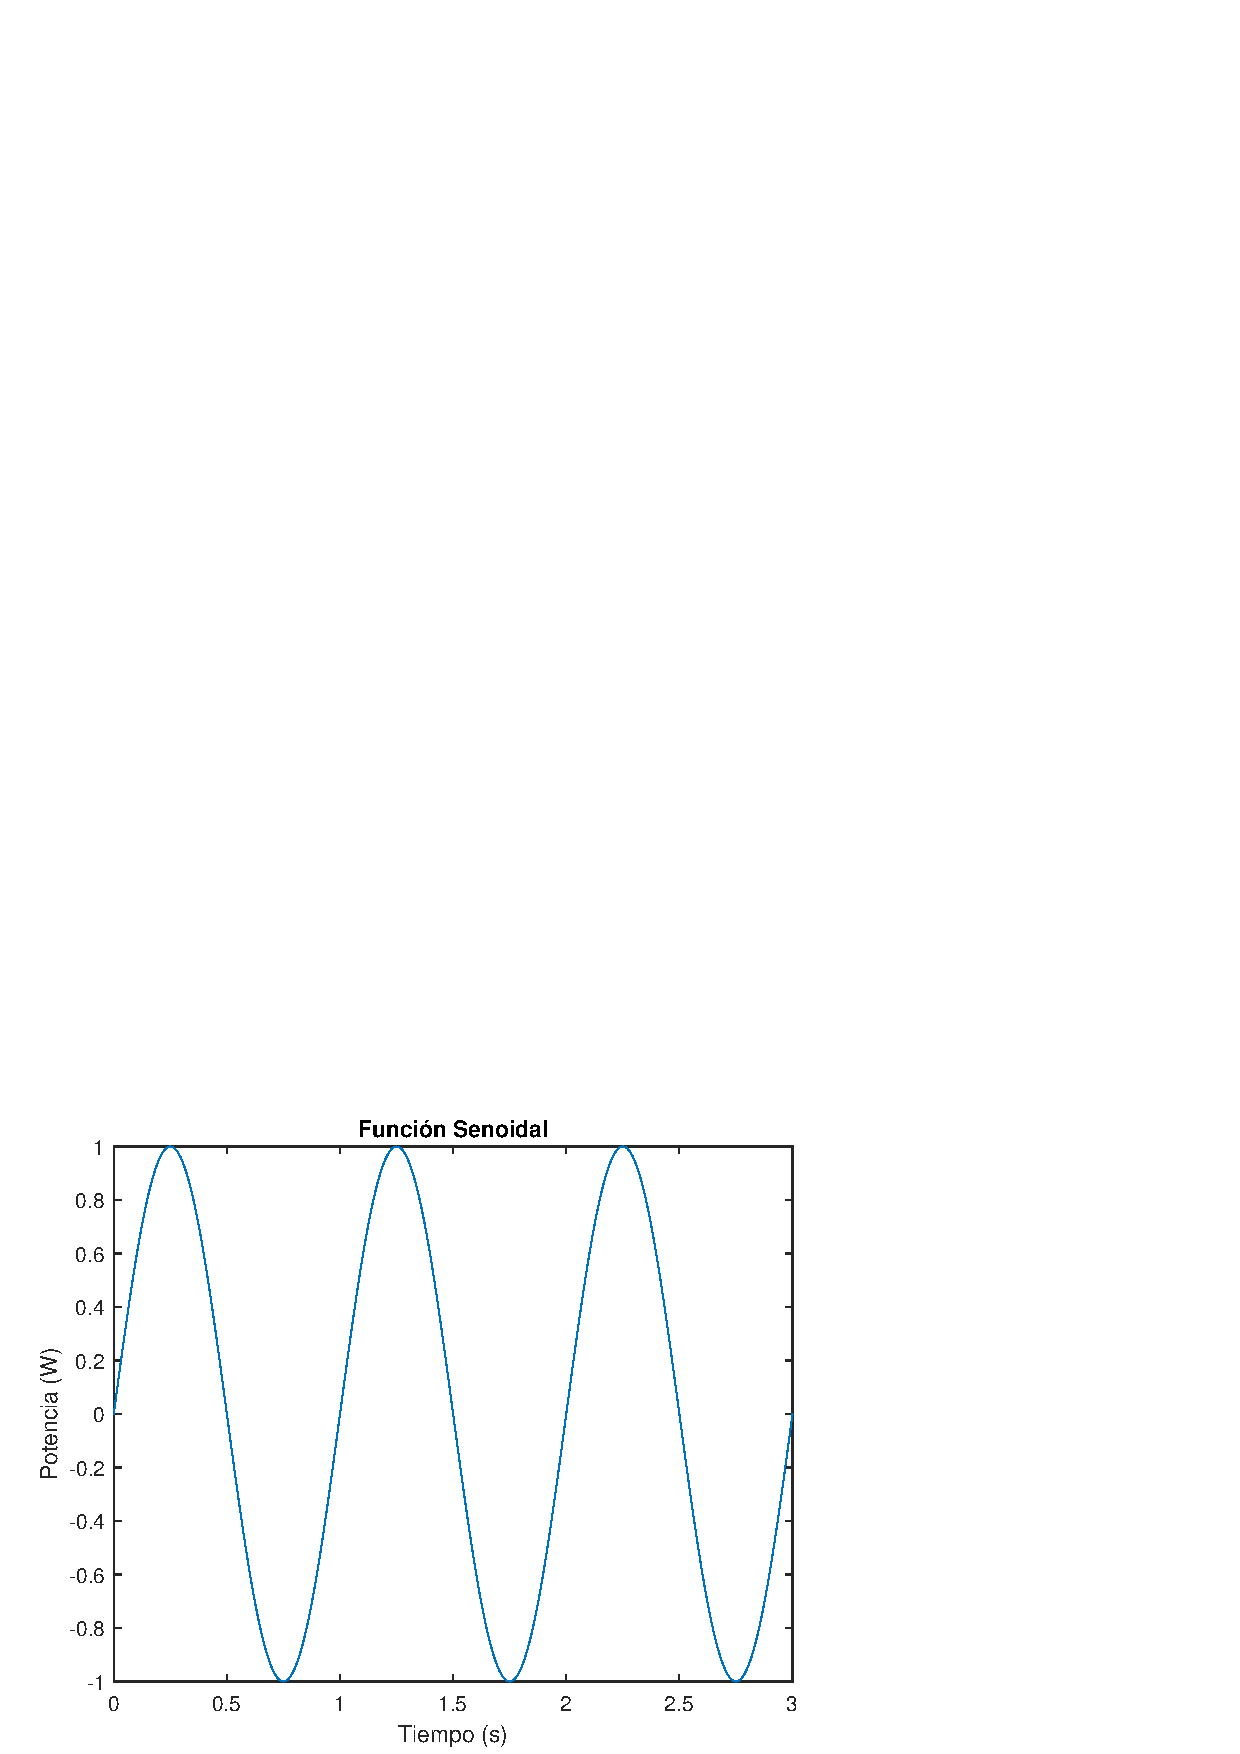
\includegraphics[width=15cm]{archivos/seno}
        \caption{Ejemplo de funcion senoidal}
        \label{fig:seno}
\end{figure}




